\chapter{LFT: Real Physics on the Lattice}\label{ch:realPhys}

We are now in a position to start tackling some real-world physics using the
methods of LFT. Nowadays lattice calculations inform many branches of particle
physics where ab initio, non-perturbative investigations are useful, for example
when computing CKM matrix elements, when exploring the QCD phase diagram at
low-to-moderate temperature near zero quark chemical potential, hadron
spectroscopy, or learning about the muon anomalous magnetic moment, just to name
a few applications.

It is common in these calculations to set $m_u=m_d\equiv m_l$.
This leads to a small systematic error, because of course the up-
and down-quark masses are not exactly equal in the real world. For most
LQCD calculations this systematic error can be neglected, but for the
highest precision measurements, for instance when calculating
the muon anomalous magnetic moment, they can comprise a substantial fraction of
the overall uncertainty. When it is relevant, this uncertainty
is referred to as\index{strong isospin breaking} {\it strong isospin breaking}.

\section{QCD thermodynamics}\label{sec:QCDtherm} 

This section focuses on the phenomenology I worked on as a postdoc in
Bielefeld, i.e. the phase diagram of QCD. There are many useful reviews
on the market, for instance Ref.~\cite{ding_thermodynamics_2015}.

In the following we will focus on $N_f=2+1$ QCD using HISQ fermions. We are
interested in nonzero $\mu$, which is not accessible directly by the lattice.
One possible strategy is to expand in small $\muh\equiv\mu/T$. For the
pressure, we find\footnote{Note that this combination on the LHS of 
\equatref{eq:pxpac} is unitless. This is because area has units
MeV$^{-2}$ and force has units MeV$^2$.}
\begin{equation}\label{eq:pxpac}
\frac{P}{T^4}=\sum_{ijk}\frac{1}{i!j!k!}\,\chi_{ijk}^{(u)(d)(s)}(T)\,
               \muh_u^i\,\muh_d^j\,\muh_s^k,
\end{equation}
where we have defined the {\it generalized
susceptibility}\index{generalized susceptibility}
\begin{equation}
\chi_{ijk}^{(u)(d)(s)}(T)
  \equiv\frac{\partial^{\,i+j+k}\,P/T^4}{\partial\muh_u^i\partial\muh_d^j
                                       \partial\muh_s^k}\Big|_{\muh=0}.
\end{equation}
Some example generalized susceptibilities could be
\begin{equation}
  \chi_2^u=\frac{\partial^2}{\partial\muh_u^2}\frac{P}{T^4}
  ~~~~\text{or}~~~~
  \chi_{11}^{us}=\frac{\partial^2}{\partial\muh_u\partial\muh_s}\frac{P}{T^4}.
\end{equation}

Another set of useful relations is between chemical potentials in the flavor
$(u,d,s)$ basis and the conserved charge $(B,Q,S)$ basis\footnote{Yet a further
possible basis of conserved charges is the $(B,I,S)$ basis with isospin $I\equiv I_3$.
For the purpose of distinguishing between $u$ and $d$ quarks only, one can use
either $I$ or $Q$.
To learn more in detail about isospin, see \secref{sec:isohyper}.}, i.e. the basis
of baryon number, electric charge, and strangeness. These relations 
are\footnote{A mnemonic to remember these relations is to ask what each quark
contributes to a system. For example a strange quark makes 1/3 of a baryon,
adds charge -1/3, and subtracts 1 from the strangeness.}
\begin{equation}\begin{aligned}\label{eq:quark-conservedCharge}
  \mu_u &= \frac{1}{3}\mu_B + \frac{2}{3}\mu_Q\\
  \mu_d &= \frac{1}{3}\mu_B - \frac{1}{3}\mu_Q\\
  \mu_s &= \frac{1}{3}\mu_B - \frac{1}{3}\mu_Q - \mu_S.
\end{aligned}\end{equation}
These relations are needed whenever one is interested in {\it conserved
charge fluctuations}\footnote{These are also sometimes referred to
as {\it generalized susceptibilities}\index{susceptibility!generalized}
or {\it cumulants}\index{cumulant}.},\index{conserved charge fluctuation} 
i.e. susceptibilities like
\begin{equation}
\chi_{ijk}^{(B)(Q)(S)}(T)
  \equiv\frac{\partial^{\,i+j+k}\,P/T^4}{\partial\muh_B^i\partial\muh_Q^j
                                       \partial\muh_S^k}\Big|_{\muh=0}.
\end{equation}
Since none of the conserved charges appears directly in the action, one
instead must decompose a conserved charge derivative into quark derivatives
using \equatref{eq:quark-conservedCharge}. For example 
one finds
\begin{equation}
  \pdv{\mu_B}
   =\sum_f\pdv{\mu_f}{\mu_B}\pdv{\mu_f}
   =\frac{1}{3}\sum_f\pdv{\mu_f}.
\end{equation}

Once we've picked a discretization, we know the action. From the perspective of
practical calculations coming from lattices, it is hence desirable to express
these formulae in terms of the partition function $Z$. From~\equatref{eq:pgrand}
we have
\begin{equation}
  \frac{P}{T^4}=\frac{1}{VT^3}\log Z,
\end{equation}
where as usual $V=(aN_s)^3$ and $T=1/aN_\tau$.
Hence we can instead
express generalized susceptibilities as
\begin{equation}
\chi_{ijk}^{(u)(d)(s)}(T)
  =\frac{1}{VT^3}\frac{\partial^{\,i+j+k}}{\partial\muh_u^i\partial\muh_d^j
                                       \partial\muh_s^k}\log Z\,\Big|_{\muh=0}.
\end{equation}

When there are $N_f$ flavors and when we use the HISQ action we have,
according to \equatref{eq:HISQdist},
\begin{equation}
  Z=\int\DD U\prod_f (\det D_f)^{1/4}\,e^{-S_G}
\end{equation}
and compute expectation values of the observable $X$ as
\begin{equation}\label{eq:HISQev}
  \ev{X}=\frac{1}{Z}\int\DD U\prod_f(\det D_f)^{1/4}\,e^{-S_G}X.
\end{equation}

Recall that in the grand canonical ensemble, a particle number
$N$ enters\footnote{See \equatref{eq:fugacity}.} 
the Boltzmann factor as $\mu N/T$; so a particle number density 
for a quark flavor $f$ is extracted as\footnote{This is consistent
with \equatref{eq:1stlawgrand}; the factor $T$ switching from
$\mu$ to $\muh$ is compensated in the definition of $\Phi$.}
\begin{equation}\label{eq:nfdensity}
  \frac{1}{V}\,\partial_{\muh_f}\log Z
  =\frac{1}{VZ}\,\partial_{\muh} Z
  =\ev{n_f}.
\end{equation}
In the staggered formulation, all the dependence on $\muh_f$ will be
hidden in $D_f$, so for $f\neq g$ we get
\begin{equation}
  \partial_{\muh_f}D_g = 0.
\end{equation}
Finally we note that, for the purpose of doing Taylor series expansions, it is
useful to remember that the QCD partition function should be blind to charge
conjugation at $\mu_B=0$. This tells us that we should expect only even powers
of $\mu_B$ when using that as the expansion parameter. 

\subsection{Derivative formulae}

We will now derive some formulae which are useful for calculations in QCD
thermodynamics. You can find even more useful formulae for a system of 
$N_f$ identical
fermion flavors in the appendix of Ref.~\cite{allton_thermodynamics_2005}.
For these calculations we will often use
\thmref{thm:exptrlog} along with \propref{prp:MATwrtSCLinv}
and \propref{prp:MATwrtSCLpowerRule}.

Our goal is to eventually take derivatives of expectation values, so from
\equatref{eq:HISQev} we will need $\muh$-derivatives of the partition 
function. For the following few formulae 
I will assume arbitrarily many non-degenerate
fermion flavors\footnote{I find this helpful to get prefactors that appear
in terms in, e.g., $\chi_2^u$ correct.}. Assuming $S_G$ has no 
$\muh$-dependence, we find
\begin{equation}
  \partial_{\muh}Z = \frac{1}{4}\sum_f 
                      Z\ev{\tr D_f^{-1}\partial_{\muh}D_f}.
\end{equation}
Hence 
\begin{equation}\label{eq:dZinv}
  \partial_{\muh}Z^{-1} = -Z^{-2}\partial_{\muh}Z
                        =\frac{1}{4}\sum_fZ\ev{\tr D_f^{-1}\partial_{\muh}D_f}
\end{equation}
and
\begin{equation}\label{eq:dlogZ}
  \partial_{\muh}\log Z=\frac{1}{4}\sum_f\ev{\tr D_f^{-1}\partial_{\muh}D_f}.
\end{equation}
Comparing \equatref{eq:dlogZ} with \equatref{eq:nfdensity} we find in
the staggered formulation
\begin{equation}
  n_f=\frac{1}{4V}\tr D_f^{-1}\partial_{\muh_f}D_f.
\end{equation} 
Finally using \equatref{eq:dZinv} one quickly derives the following useful formula
for an observable $O$ calculated on HISQ configurations:
\begin{proposition}{}{dO}
\begin{equation*} \partial_{\muh}\ev{O}
       =   \ev{\partial_{\muh}O}
        -\frac{1}{4}\sum_f\ev{\tr D_f^{-1}\partial_{\muh}D_f}\ev{O}
         +\frac{1}{4}\sum_f\ev{O\tr D_f^{-1}\partial_{\muh}D_f}
\end{equation*}
\end{proposition} 
Note that if $\muh=\muh_f$ with $N_f$ degenerate flavors, 
\propref{prp:dO} reduces to eq.~(A3)
in Ref.~\cite{allton_thermodynamics_2005}. Using this Proposition along
with \equatref{eq:dlogZ}, one 
can start expressing generalized susceptibilities in terms of the fermion
matrix. For example one finds for any flavor $f$
\begin{equation}\begin{aligned}
  VT^3\,\chi_2^f =\partial_{\muh_f}^{\,2}\log Z
                 =\, & \frac{1}{16}\ev{\left(\tr D_f^{-1}D_f'\right)^2}
                    -\frac{1}{16}\ev{\tr D_f^{-1}D_f'}^2\\
                   & -\frac{1}{4}\ev{\tr \left(D_f^{-1} D_f'\right)^2}
                    +\frac{1}{4}\ev{\tr D_f^{-1}D_f''},
\end{aligned}\end{equation}
where a prime on $D_f$ indicates a derivative w.r.t. the corresponding chemical
potential $\muh_f$. Similarly for two flavors $f\neq g$ 
\begin{equation}\begin{aligned}
  VT^3\,\chi_{11}^{fg} =\partial_{\muh_f}\partial_{\muh_g}\log Z
                 = \,& \frac{1}{16}\ev{\tr D_f^{-1}D_f'\tr D_g^{-1}D_g'} \\
                   & -\frac{1}{16}\ev{\tr D_f^{-1}D_f'}\ev{\tr D_g^{-1}D_g'}.
\end{aligned}\end{equation}
Using an $N_f=2+1$ HISQ action with $m_l\equiv m_u=m_d$ along with 
\equatref{eq:quark-conservedCharge}, one can figure out how to 
express\footnote{Note that when carrying out calculations like these, to avoid making mistakes,
one should always work with non-degenerate flavors, then allow the flavors to be
degenerate at the end. This way one correctly distinguishes between e.g.
$\chi_{11}^{ll}$ and $\chi_2^l$.} conserved charge fluctuations in terms of 
generalized susceptibilities, such as
\begin{equation}\begin{aligned}\label{eq:2ndorderdiagonal}
  \chi_2^B&=\frac{1}{9}\left(2\chi_2^l+\chi_2^s+2\chi_{11}^{ll}+4\chi_{11}^{ls}\right)\\
  \chi_2^Q&=\frac{1}{9}\left(5\chi_2^l+\chi_2^s-4\chi_{11}^{ll}-2\chi_{11}^{ls}\right)\\
  \chi_2^S&=\chi_2^s.
\end{aligned}\end{equation}
Sometimes we call cumulants with derivatives of only one variety
{\it diagonal} cumulants\index{cumulant!diagonal}; hence
\equatref{eq:2ndorderdiagonal} lists all second-order, diagonal cumulants.
Expressions for the second-order, off-diagonal cumulants are
\begin{equation}\begin{aligned}
\chi^{QS}_{11}&=\frac{1}{3}\left(\chi^{s}_{2}-\chi^{ls}_{11}\right)\\
\chi^{BS}_{11}&=\frac{1}{3}\left(-\chi^{s}_{2}-2\chi^{ls}_{11}\right)\\
\chi^{BQ}_{11}&=\frac{1}{9}\left(\chi^{l}_{2}-\chi^{s}_{2}+\chi^{ll}_{11}-\chi^{ls}_{11}\right).
\end{aligned}\end{equation}




\subsection{QCD material parameters}


The speed of sound at fixed control parameter $X$ is defined as
\begin{equation}
  c_X^2=\left(\pdv{p}{\epsilon}\right)_X.
\end{equation}
In a simple (1+1)-$d$ isotropic model of a heavy ion collision, 
sometimes referred to as \index{Bjorken flow}{\it Bjorken flow}, 
assuming a constant $c_s^2$, one can show~\cite{bjorken_highly_1983} 
that the energy density will decrease with proper time $\tau$ as
\begin{equation}
  \epsilon(\tau)=\epsilon(\tau_0)\left(\frac{\tau_0}{\tau}\right)^{1+c_s^2}.
\end{equation}
In this picture one thus finds the system cools with longitudinal expansion
of the fireball according to the speed of sound. % Henrik's thesis is nice
Also in the context of heavy ion collisions, it can be used to look out
for a long-lived fireball, which may coincide with a {\it softest point}
\index{softest point} where the pressure-to-energy-density ratio,
and hence $c_s^2$, attains a minimum\footnote{Another way of looking at
this is that near the crossover as we increase temperature, this
energy serves to change hadronic degrees of freedom to screened
quarks and gluons, rather than changing the pressure.}~\cite{hung_hydrodynamics_1995}.
In the context of neutron stars, $c_s^2$ is interesting since the relationship
between the star masses and radii is influenced by how $c_s^2$ changes with
$n_B$~\cite{ozel_masses_2016}.

The speed of sound has been calculated at $\mu_B=0$ on the 
lattice~\cite{borsanyi_qcd_2010,bazavov_equation_2014,borsanyi_full_2014}.
It has also been calculated using PNJL and NJL 
\index{NJL model}\index{PNJL model}
models\footnote{The Nambu-Jona-Lasinio (NJL)
model~\cite{nambu_dynamical_1961,nambu_dynamical_1961-1} is a low-energy,
effective model of interacting chiral fermions, i.e. it has a 4-fermion
interaction term. This means it's non-renormalizable, so it is not expected
to be a correct description at very high energies.
In the Polyakov-loop-extended NJL (PNJL) model~\cite{meisinger_chiral_1996}, 
one includes the zeroth component of the gauge field. The field is assumed to
be spatially uniform.}~\cite{ghosh_susceptibilities_2006,marty_transport_2013,deb_estimating_2016,motta_isentropic_2020,zhao_thermodynamic_2020};
in the quark-meson coupling
model~\cite{schaefer_thermodynamics_2010,abhishek_transport_2018};
the field correlator
method~\cite{khaidukov_speed_2018,khaidukov_thermodynamics_2019};
and in the quasiparticle method~\cite{mykhaylova_impact_2021}.

\section{The QCD phase diagram}

\begin{figure}
\centering
\vspace{-1cm}
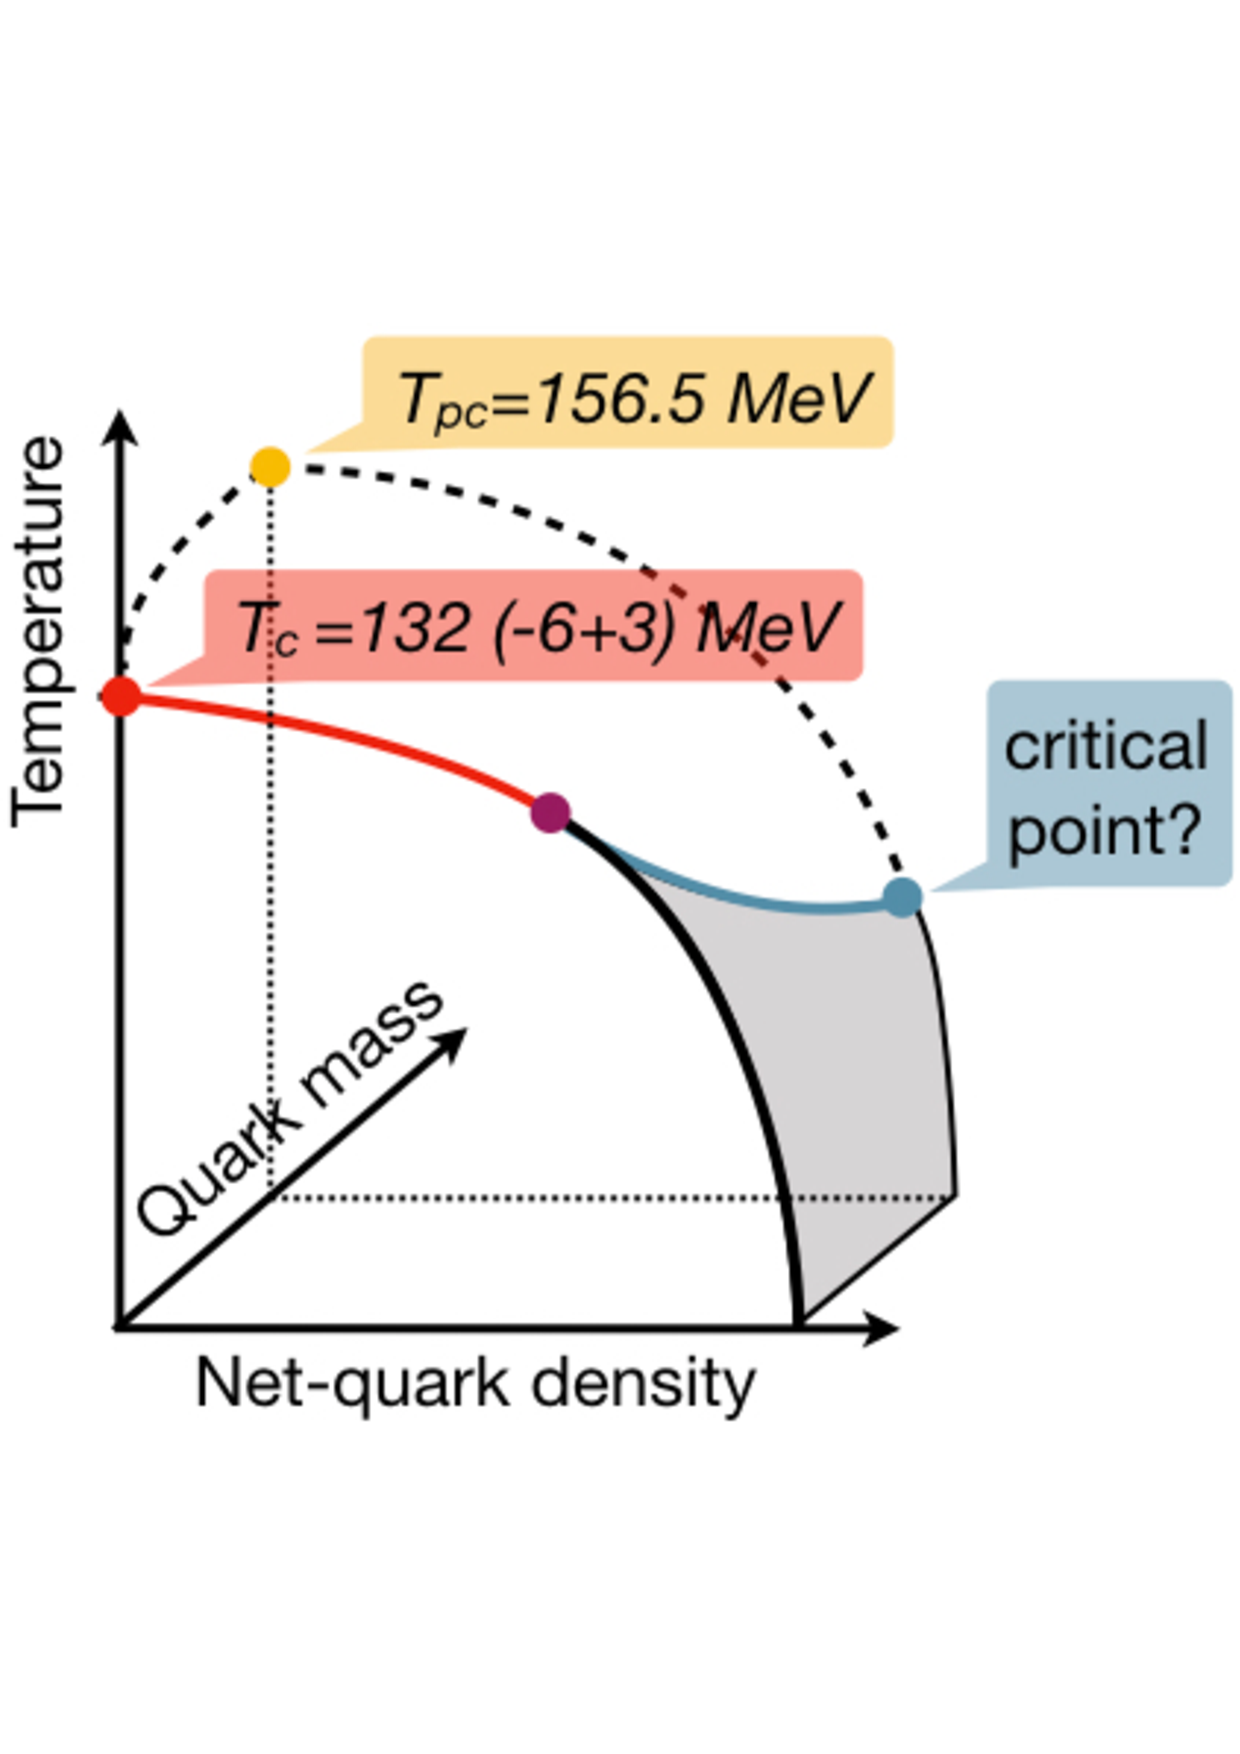
\includegraphics[width=0.48\linewidth]{figs/3d_phase_diag_Gauss.003.pdf}
\hspace{-2mm}
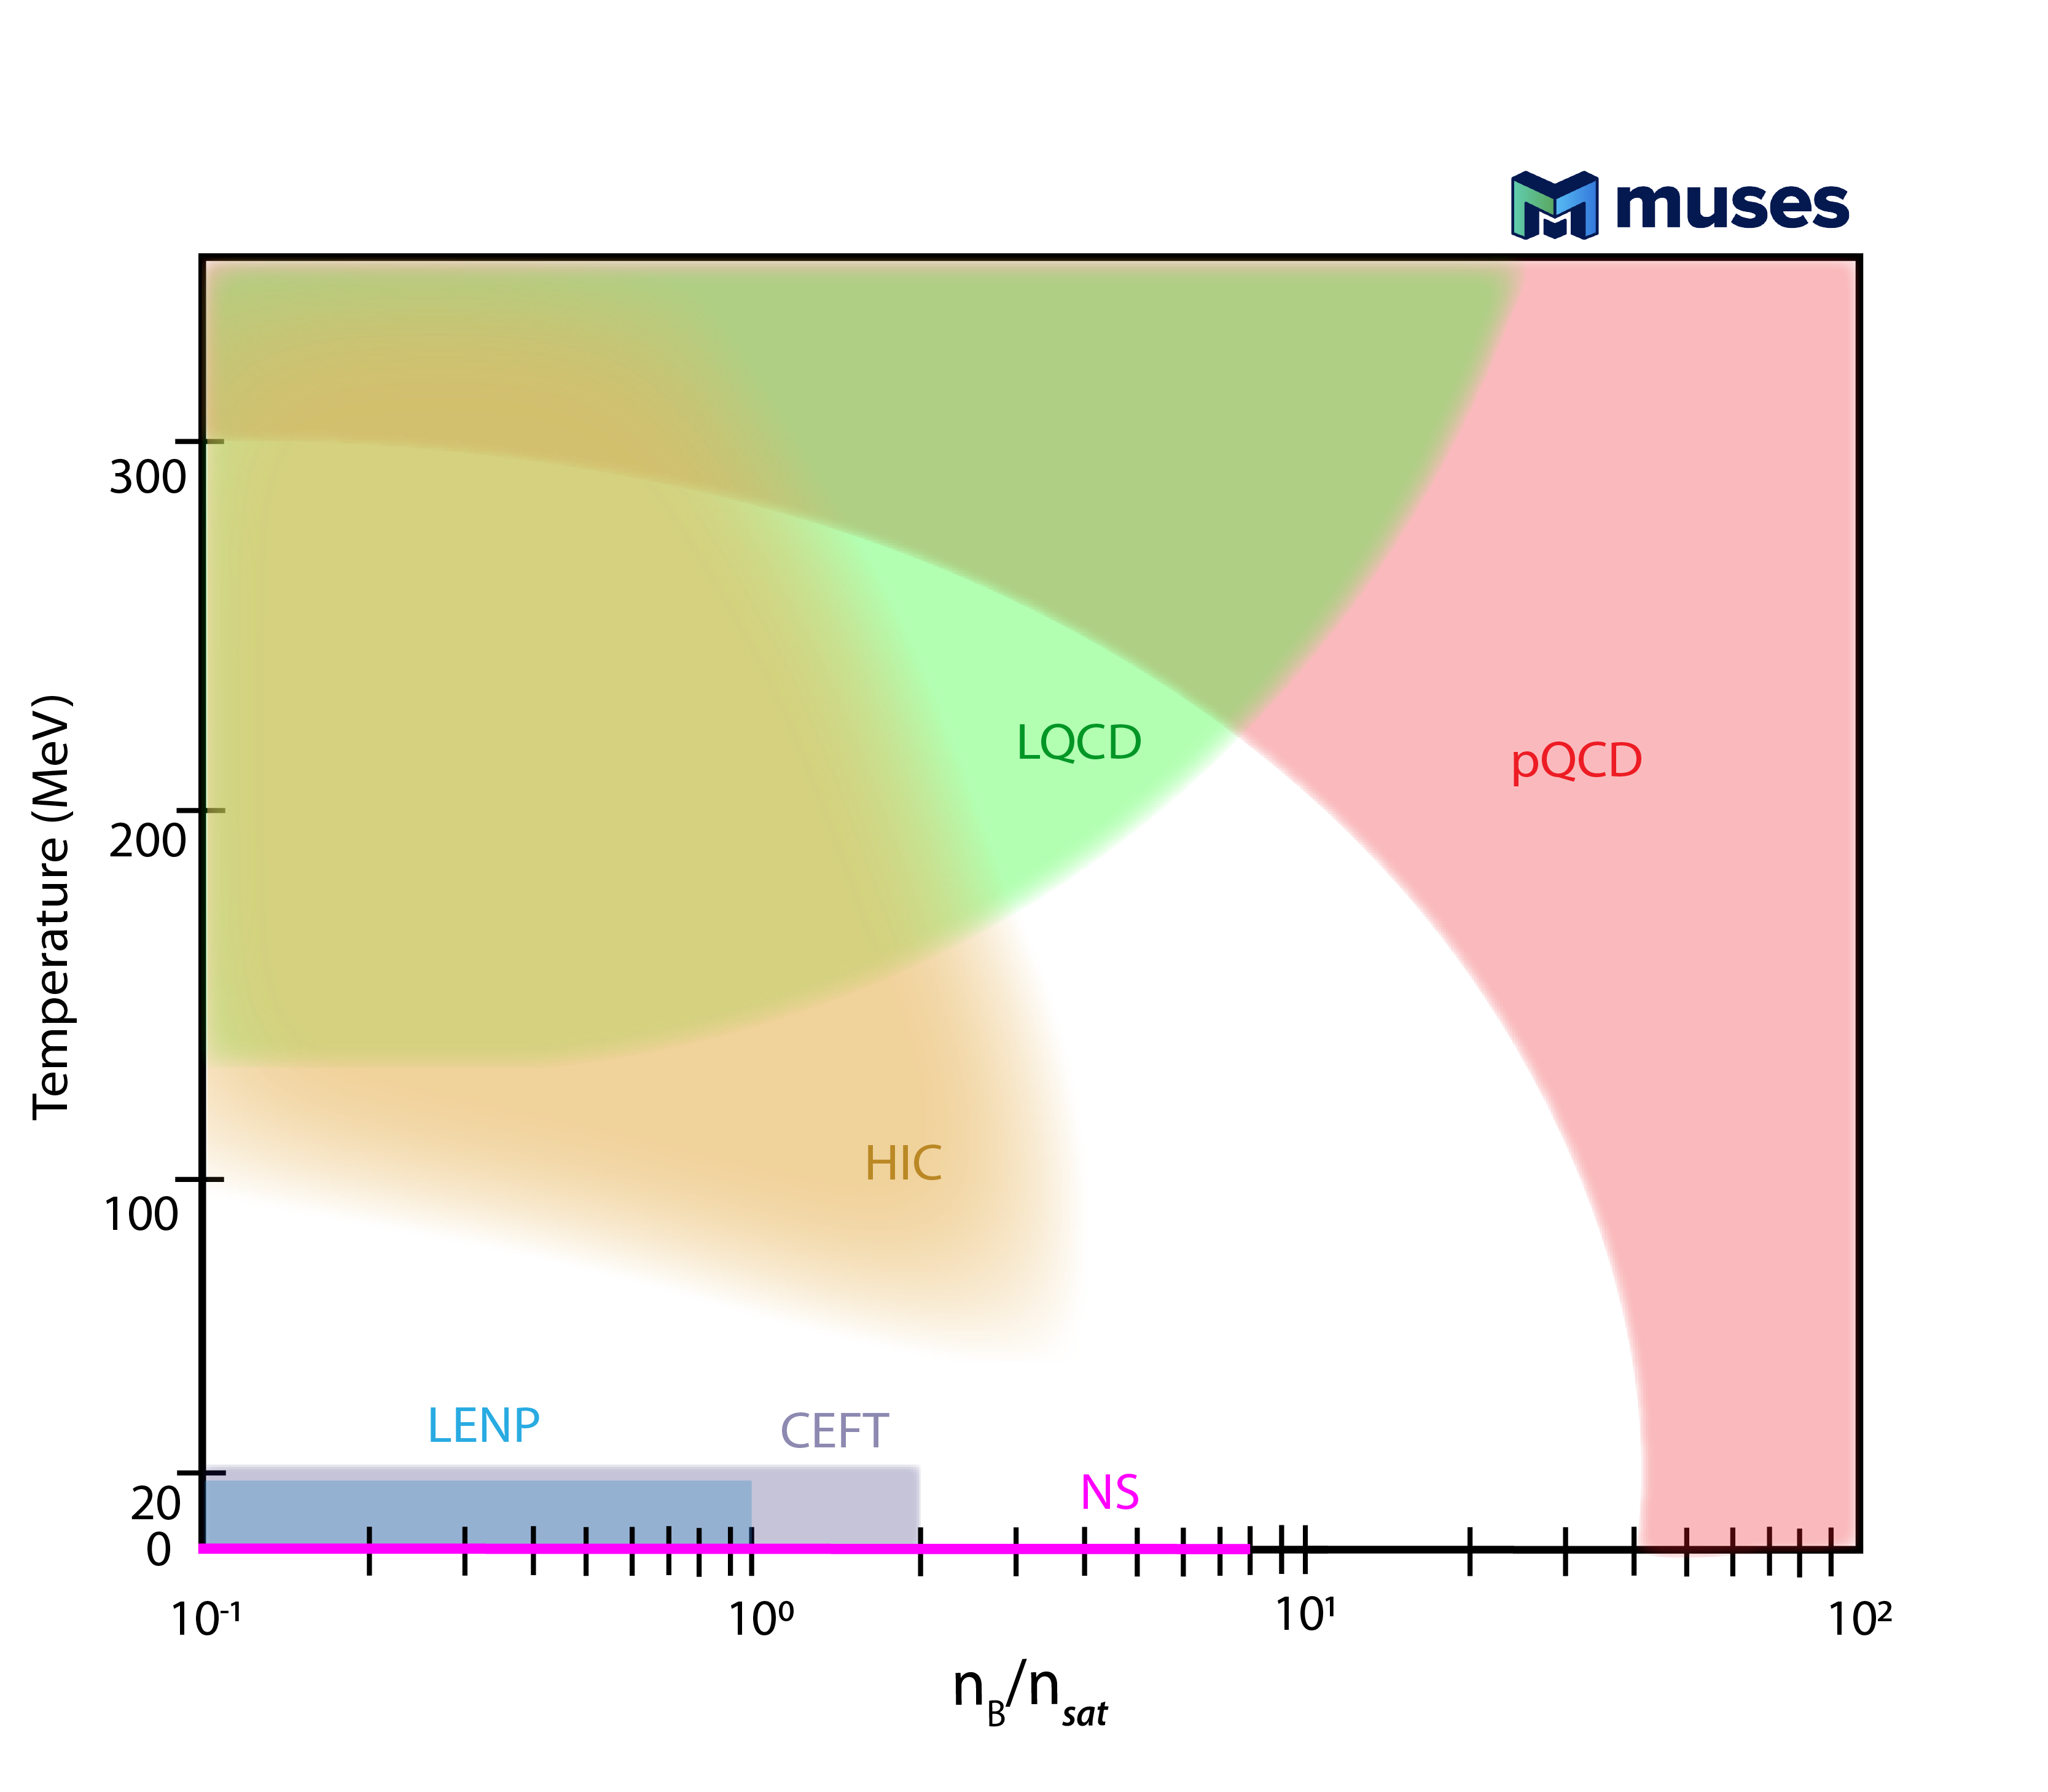
\includegraphics[width=0.48\linewidth]{figs/accessibleQCD.png}
\caption{{\it Left}: Schematic phase diagram of QCD. Indicated are the pseudocritical 
transition temperature $\Tpc$ of QCD at physical quark mass and the critical 
transition temperature $\Tc$ in the chiral limit. Dashed lines indicate 
crossovers; thick, solid, colored lines are lines of second-order phase 
transitions; the thick, solid, black line is a line of first-order
transitions; and a first-order surface is indicated in grey. 
A possible critical endpoint is indicated in teal. Figure by C. Schmidt.
This figure is described in more detail in Ref.~\cite{karsch_critical_2019}.
{\it Right}: QCD phase diagram against net baryon-number density at
physical quark mass. 
Here we schematically see regions of applicability of several approaches
to understanding QCD matter. Figure from the MUSES 
collaboration~\cite{MUSES:2023hyz}.
}
\label{fig:pdiag}
\end{figure}

At sufficiently high $T$ and/or $\mu_B$, nucleons dissociate into their constituents, 
and nuclear matter changes phase from a gas of hadrons to quark-gluon plasma.
At low enough temperature, one eventually encounters with increasing $\mu_B$ a line of 
first-order transitions, which is expected to terminate at a second-order critical 
endpoint belonging to the 3-$d$, $\Z_2$ universality class, as shown in the rear 
plane of Fig.~\ref{fig:pdiag}.

Let us discuss the qualitative form of the phase diagram in a bit more 
detail~\cite{halasz_phase_1998}.
At $T=0$ and physical quark masses\footnote{We are moving along the dotted,
horizontal line in the rear plane.}, it can be argued that baryon-number 
density $n_B$ should jump at
$\mu\approx m_p$ to the {\it nuclear matter density}\index{nuclear matter
density} $n_0\approx 0.16$ fm$^{-3}$. This jump is discontinuous, and
so the expectation is that transition is first-order, with $n_B$
playing the role of an order parameter.
At sufficiently large $\mu$, color interactions are expected to be screened,
and hence non-perturbative effects like global symmetry breaking should
be suppressed. So for massless quarks, one expects for large $\mu$
a chirally-restored phase, and this should also be of 
first-order\footnote{Now moving along the horizontal axis in
the foreground.}. 
When $\mu$ is sufficiently small and when $m_l=0$,
there is a second-order chiral phase transition belonging to the
$\SU(2)_L\times\SU(2)_R\cong\ON(4)$ universality class.

Returning to the first-order transition at $T=0$ and $m_l=0$,
moving off the $T=0$ axis, continuity demands
the first-order transition to continue as a line. Once $T\neq0$, there
is no longer a well-defined order parameter, and this requirement is lost;
the expectation is this terminates in a tricritical point, which is
itself connect to a second-order line. The ``wings" of this tricritical
point branch off to second-order lines at positive and negative quark
mass\footnote{There is a $m_l\to-m_l$ symmetry, which is not indicated
in the figure since only $m_l\geq0$ is shown.}.

Let us now think about how to probe this diagram on the lattice.
When viewed from the plane of complex $\muh$, the Taylor expansion 
approach is limited by the location of the nearest zero of the QCD partition 
function $\ZQCD$, i.e. the nearest singularity of the free energy in the 
complex plane. In terms of the universal scaling in the vicinity of a critical 
point, the nearest singularity might be identified with the Lee-Yang 
edge, as discussed in \secref{sec:leeyang}. Thus understanding the analytic 
structure of the $\log\ZQCD$ gives crucial insight on both
the convergence radius of these $\muh$-expansions and universal critical behaviour 
in the vicinity of the phase transitions.


\subsection{The sign problem}\index{sign problem}\label{sec:signProblem}


Unfortunately at $\mu_B>0$, the Boltzmann factor becomes complex, and a 
direct estimate of the path 
integral through MCMC is no longer possible--this is the infamous {\it sign problem}.
This limitation is a special hindrance when looking out for the possible critical 
endpoint at nonzero $\mu_B$ mentioned above. 
Nevertheless many approaches have been developed to at least partially circumvent this limitation, 
each with its own merits, drawbacks, and regions of applicability.
Two popular approaches include Taylor expansions of the equation of state in 
$\muh\equiv\mu_B/T$~\cite{Allton:2002zi, Allton:2003vx, Gavai:2003mf} and analytic continuation 
from purely imaginary chemical potential  $\muh=i\muh_I$~\cite{deForcrand:2002hgr, DElia:2002tig}.

Let us try to understand this problem in more detail.
Most\footnote{Dirac operators with a $\theta$ angle, a twisted mass,
or as we shall shortly see, a chemical potential, lose this property.} 
commonly used Dirac operators $D$ are
$\gamma_5$-{\it hermitian}\index{hermitian}, i.e. they satisfy
\begin{equation}
\gamma_5 D\gamma_5=D^\dagger.
\end{equation}
We already know that hermitian matrices have real eigenvalues, which
is a reason why we like them. 
\begin{proposition}{}{}
Eigenvalues of $\gamma_5$-hermitian matrices come in complex-conjugate pairs.
Moreover their determinants are real.
\begin{proof}
Let $D$ be $\gamma_5$-hermitian. Then since $\gamma_5^2=\id$,
\begin{equation*}\begin{aligned}
\det\left(D-\lambda\id\right)
&=\det\left(\gamma_5^2\left(D-\lambda\id\right)\right)\\
&=\det\left(\gamma_5\left(D-\lambda\id\right)\gamma_5\right)\\
&=\det\left(D^\dagger-\lambda\id\right)\\
&=\det\left(D-\lambda^*\id\right)^*,\\
\end{aligned}\end{equation*}
which shows the first statement. The next statement uses basically
the same trick, i.e.
$$
\det D 
= \det\left(\gamma_5^2 D\right) 
= \det\left(\gamma_5 D\gamma_5\right) 
= \det D^\dagger
= \det D^*.
$$
\end{proof}
\end{proposition}

These kinds of tricks let us see one way the sign problem manifests.
When we introduce a chemical potential, it couples to $\gamma_4$.
Thus a Dirac operator with a chemical potential obeys
\begin{equation}\label{eq:signproblem}
\det\left(D-\mu\gamma_4\right)
=\det\left(\gamma_5\left(D-\mu\gamma_4\right)\gamma_5\right)
=\det\left(D+\mu^*\gamma_4\right)^*
\end{equation}
from which it follows that
$\det\left(D-\mu\gamma_4\right)\in\R$ if and only if $\mu$
is pure imaginary. Hence at real $\mu$, the determinant
is complex. On the other hand, the determinant of the
Dirac operator is part of the probability weight
of the partition function, which one sees explicitly for
the HISQ action in \equatref{eq:HISQdist}. If this
determinant is not strictly real, its interpretation
as a PDF becomes nonsensical.

There is no complete solution to the sign problem. Still, there are
some workarounds that enjoy various degrees of success.
One of the most straightforward is hinted at by
\equatref{eq:signproblem}; namely there is no sign problem
if we simulate at pure imaginary $\mu$. Under the assumption
that we simulate within the convergence radius of our
observable of interest, we can then in principle analytically
continue from the imaginary axis to the real one.

{\it Reweighting}~\cite{ferrenberg_new_1989}\index{reweighting}
is another possibility. One can reweight in any parameter that
enters linearly in the action. 
We showcase the idea by doing reweighting in $\beta=1/T$ for
an arbitrary statistical physics theory of some field $\phi$. Consider
the expectation value of an observable $X$ calculated at $\beta'$. We have
\begin{equation}
\begin{aligned}
  \ev{X}_{\beta'}&=Z_{\beta'}^{-1}\int\dd{\phi}e^{-\beta'E(\phi)}X(\phi)
                  e^{(\beta-\beta)E(\phi)}\\
                 &=Z_{\beta'}^{-1}\int\dd{\phi}e^{(\beta-\beta')E(\phi)}
                  X(\phi)e^{-\beta E(\phi)}\\
                 &=Z_{\beta'}^{-1}Z_{\beta}\ev{e^{(\beta-\beta')E}X}_\beta.
\end{aligned}
\end{equation}
To determine the factor $Z_{\beta'}^{-1}Z_{\beta}$, just plug in $X=1$.
One finds
\begin{equation}
Z_{\beta'}^{-1}Z_{\beta}=\ev{e^{(\beta-\beta')E}}_{\beta}^{-1},
\end{equation}
and so
\begin{equation}\label{eq:RW}
\ev{X}_{\beta'}=\frac{\ev{e^{(\beta-\beta')E}X}_\beta}{\ev{e^{(\beta-\beta')E}}_{\beta}}.
\end{equation}


We can calculate the expectation value in the last line
using data from a time series generated at $\beta$, and this gives us an
estimate for $\ev{X}_{\beta'}$. Reweighting is only useful when
$E\Delta\beta=\order{1}$. Since $E$ is extensive, this leads to the
expectation that the range of $\beta$ where reweighting gives reliable
information is suppressed for large volumes. 
Provided that the critical parameter $\beta_c$
is sufficiently close to the simulation point $\beta$, it suffices
to have only one simulation, estimating the maximum by reweighting to
multiple nearby $\beta'$. This strategy can be similarly applied
to a chemical potential $\mu$, but the limitation is the same: as
the volume increases the range where one can extract reliable
information gets squeezed.

The Taylor series approach introduced earlier can also be used to
glean some information at $\mu_B>0$. The idea here is that each
coefficient of the Taylor series is by definition computed at
$\mu_B=0$, which can be handled on the lattice. Then assuming
$\mu_B/T$ is small enough, the expansion of some observable in
$\mu_B/T$ ought to be a reasonable approximation.

\index{Roberge-Weiss transition}
\subsection{The Roberge-Weiss transition}\label{sec:RW}



\section{The muon anomalous magnetic moment}\label{sec:muonAnom}

This chapter focuses on some phenomenology I worked on as a postdoc at Utah.
An overview of lattice and dispersive approaches to this problem can
be found in, e.g., Ref.~\cite{aoyama_anomalous_2020}.

The motivation to study the muon anomalous magnetic moment is pretty
straightforward: Observations such as the existence of dark matter and
dark energy cannot be explained by any SM phenomena. One possibility to probe
for new physics is to increase the energy of particle accelerators, thereby
allowing experiment to access higher and higher masses--this is sometimes
called the\index{energy frontier} {\it energy frontier}.
Another possibility is to make more precise measurements, thereby revealing or
sharpening tensions between the SM and experiment--this is
the\index{intensity frontier} {\it intensity frontier}.

As already mentioned in \secref{sec:magAnom}, there is an interesting situation
where data-driven theory exhibit a mild tension with lattice results.
A strategy currently taken by the community to unravel this tension is to
implement modified observables that reduce or magnify systematic effects,
depending on what you want to examine. These are called {\it window observables}
in\index{window observable} the literature.

As an example, the leading HVP contribution $\amuhvp$ in the
{\it time-momentum representation} (TMR) is~\cite{bernecker_vector_2011}
\begin{equation}\label{eq:amuhvp}
  \amuhvp=\left(\frac{\alpha}{\pi}\right)^2\int\dd{t}\tilde{K}(t)G(t),
\end{equation}
where $G(t)$ is the spatially summed correlation function of the EM 
current\footnote{According to the notation of \secref{sec:discreteSymm}
this is a vector current.}
\begin{equation}\begin{aligned}
  G(t) &=-\frac{a^3}{3}\sum_{k=1}^3\sum_{\vec{x}}\ev{j_k(t,\vec{x})j_k(0)},\\
  j_\mu&=\sum_fq_f\bar{\psi}_f\gamma_\mu\psi_f,
\end{aligned}\end{equation}
where $q_f$ is the electric charge of the quark species $f$,
and $\tilde{K}(t)$ is a known kernel function.

In this case a window observable
can be constructed by multiplying the integrand of \equatref{eq:amuhvp} by some
function that enhances the integrand only in certain time windows of the
integral. A step function would naively do the trick, but the authors
in Ref.~\cite{blum_calculation_2018} found that the smoothed step function
\begin{equation}
  \Theta(t,t',\Delta)\equiv\frac{1}{2}\left(1+\tanh\left(\frac{t-t'}{\Delta}\right)\right)
\end{equation}
was somehow less sensitive to discretization effects.
Window observables can be used for high-precision comparisons between both
data-driven calculations and lattice calculations.

\section{Scale setting II}\label{sec:refscalesII}\index{scale!setting}

\bibliographystyle{unsrtnat}
\bibliography{bibliography}
